\chapter{Soluzione proposta - Titolo provvisorio}

\section{Introduzione}
%spiegare obiettivo
Il mio obiettivo è di creare un sistema di anomaly detection con struttura distribuita: nei router delle sedi periferiche raccolgo informazioni sul traffico e in un server posizionato fisicamente nella sede centrale lo analizzo e prendo decisioni sulle azioni da compiere. Per svolgere questo lavoro mi sono dovuto basare su alcuni software e sull'hardware aziendale con i relativi vantaggi e svantaggi rispetto ad una soluzione completamente ex-novo.
% spiegare come vengono gestiti i dati

\section{Obiettivo}

\subsection{Gestione dei dati}

I dati vengono collezionati tramite un demone sui router (collectd), inviati al server (go-graphite) e visualizzati tramite una dashboard(graphana). Il tool di anomaly detection da me pensato si interfaccia direttamente con il database per la lettura dei dati e la scrittura dei risultati.
Qui in seguito approfondirò maggiormente il flusso della gestione dei dati.

\begin{figure}[]
    % todo: capire come gestire citazioni imsmagini a livello di copyright
    %  e capire come funzionano le label per richiamare le immagini
    \label{fig:mos}
    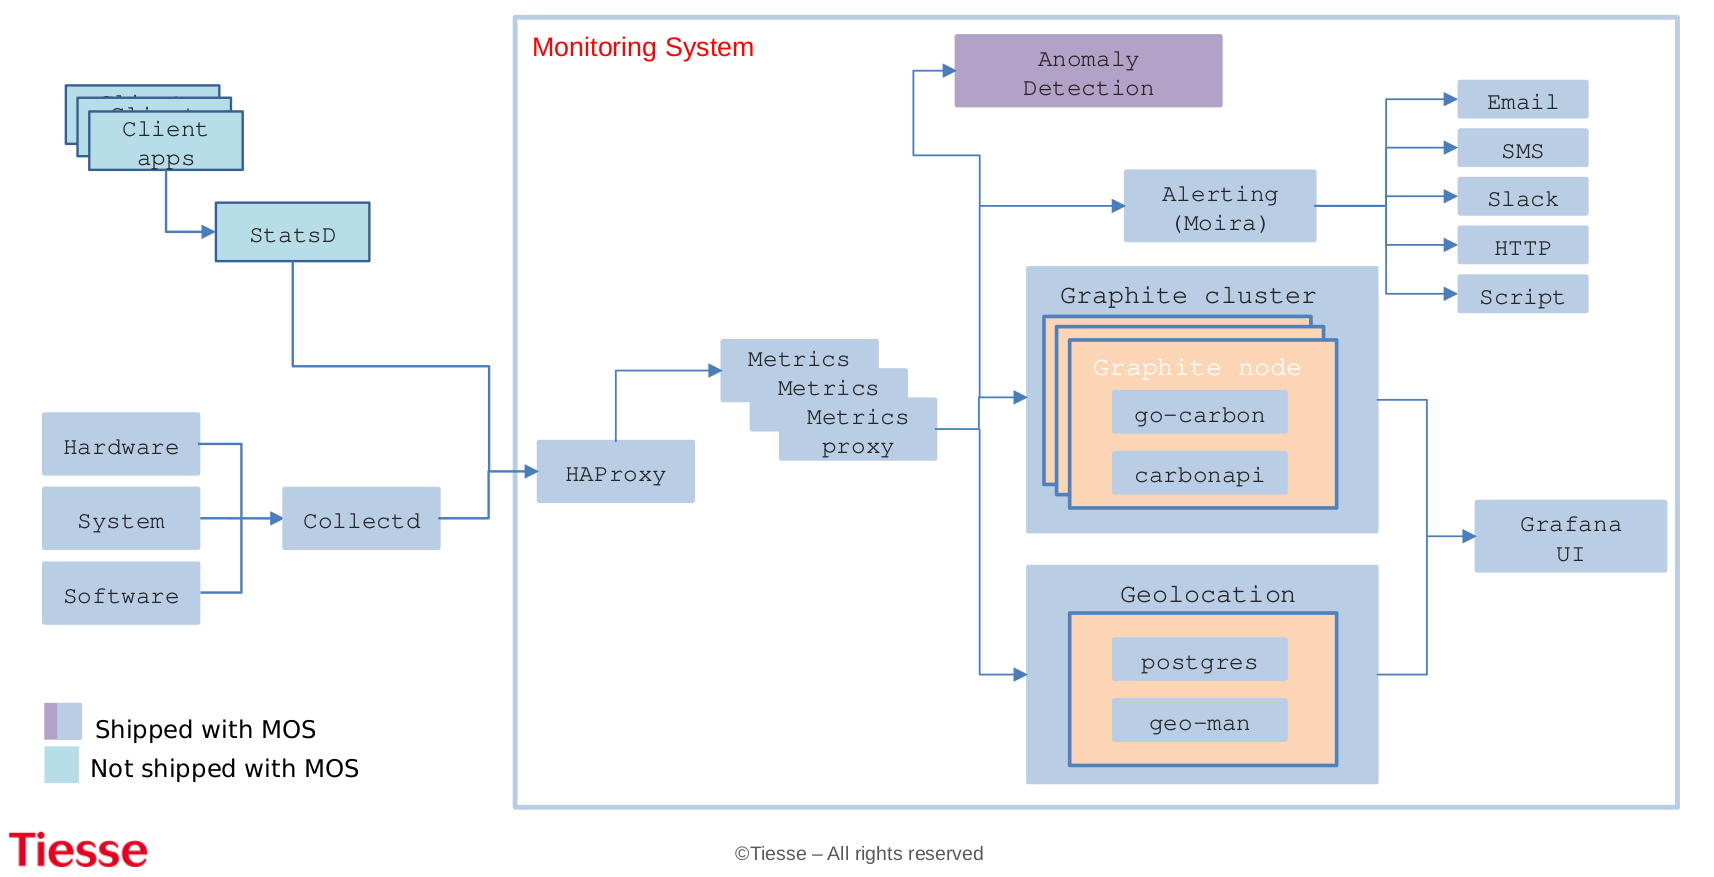
\includegraphics[width=\hsize]{images/my_work/tiesse_mos.png}
    \caption{Architettura di MOS (Monitor System di Tiesse)}
    \centering
\end{figure}

\paragraph{collectd} è un demone che raccoglie metriche di sistema e di applicazioni, trasferisce e salva dati di computer e dispositivi di rete. Collect ha una struttura modulare in cui è possibile abilitare centinaia di plugin per la raccolta di metriche di sistema dai casi più generali a quelli più specifici ed inoltre è possibile scrivere i propri plugin per integrarlo ulteriormente. I plugin da me usati sono ``write\_graphite'': plugin che permette di scrivere le metriche raccolte su un database graphite, ``conntrack'': plugin che permette di contare il numero di voci nella connection tracking table di Linux, ``interface'' : plugin che colleziona informazioni sul traffico su un'interfaccia, quindi pacchetti al secondo, bytes al secondo ed errori sull'interfaccia. 

Inoltre per avere ulteriori dati a disposizione ho scritto un plugin che si occupa di aggiungere delle metriche sul conteggio dei pacchetti non possibile con i plugin standard.

\paragraph{Il mio plugin di collect}

\paragraph{NDPI} è un software per il deep-packet inspection basato su OpenDPI
%http://luca.ntop.org/nDPI.pdf
%todo: completare ndpi

%todo: posso parlare della prima versione, dei problemi riscontrati e dell'utilizzo di ebpf al suo posto
\paragraph{graphite} è un software open source per il monitoraggio che può funzionare sia su hardware economico, che su un'infrastruttura cloud. Può essere usato per monitorare le performance di siti, applicazioni, server e nel caso di Tiesse è usato per monitorare informazioni sull'uso dei router, come per esempio il numero totale di router connessi, quelli raggiungibili, il throughput, l'uptime e la velocità della connessione xDSL.
L'obiettivo di graphite è il salvataggio di serie temporali di dati numerici e la successiva condivisione e visualizzazione.
Graphite è composto da tre parti (come si può vedere dalla figura ~\ref{fig:graphite}):

% https://www.aosabook.org/en/graphite.html
% https://graphiteapp.org/#gettingStarted
%todo: spiegare meglio come funzionano le carbon api
\begin{itemize}
    \item carbon: è un service ad altre prestazioni che si occupa di ricevere le metriche con formato ``(timestamp, value)'' da salvare.
    \item whisper: un semplice database che salva sul filesystem le sequenze temporali di dati.
    \item graphite-web: è un'interfaccia utente e delle API le quali restituiscono i dati per renderizzare i grafici da visualizzare.
\end{itemize}

\begin{figure}[h]
    % todo: capire come gestire citazioni imsmagini a livello di copyright
    %  e capire come funzionano le label per richiamare le immagini
    \label{fig:graphite}
    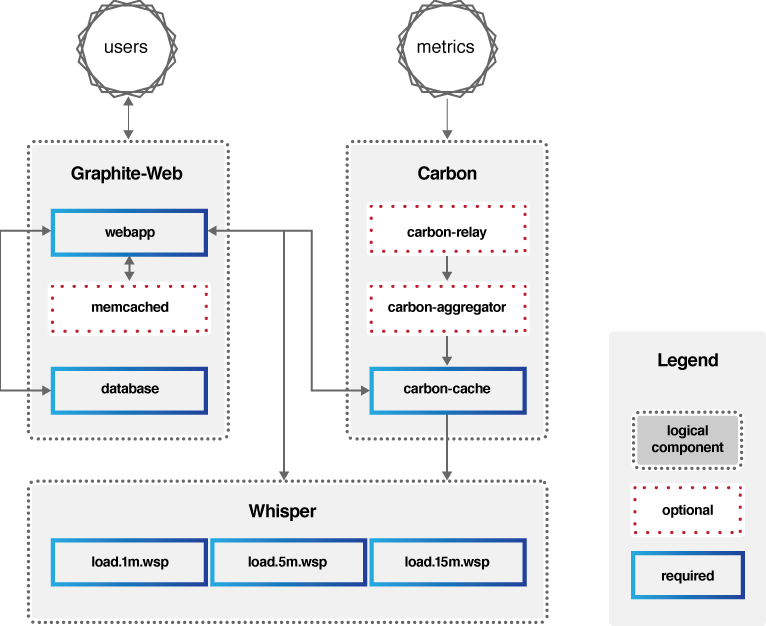
\includegraphics[width=\hsize]{images/my_work/graphite.png}
    \caption{Architettura di Graphite}
    \centering
\end{figure}

\paragraph{go-graphite} è un'implementazione in Golang di Graphite, rispetto alla versione originale di carbon il backend
go-carbon è più veloce in tutte le condizioni (la differenza di prestazioni varia in base alla macchina su cui è installato) ~\ref{fig:gocarbon}.
Le carbonapi invece sono un subset delle api di graphite-web e le vanno a sostituire essendo dalle 5 alle 10 volte più veloci.

\begin{figure}[h]
    % todo: capire come gestire citazioni imsmagini a livello di copyright
    %  e capire come funzionano le label per richiamare le immagini
    \label{fig:gocarbon}
    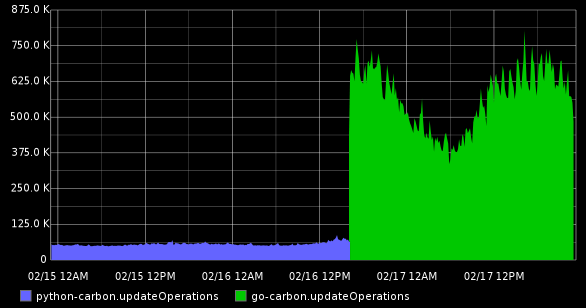
\includegraphics[width=\hsize]{images/my_work/go-carbon.png}
    \caption{Differenza di prestazioni tra carbon e go-carbon}
    \centering
\end{figure}
% https://github.com/go-graphite/go-carbon


\begin{figure}[h]
    % todo: capire come gestire citazioni imsmagini a livello di copyright
    %  e capire come funzionano le label per richiamare le immagini
    \label{fig:graphana}
    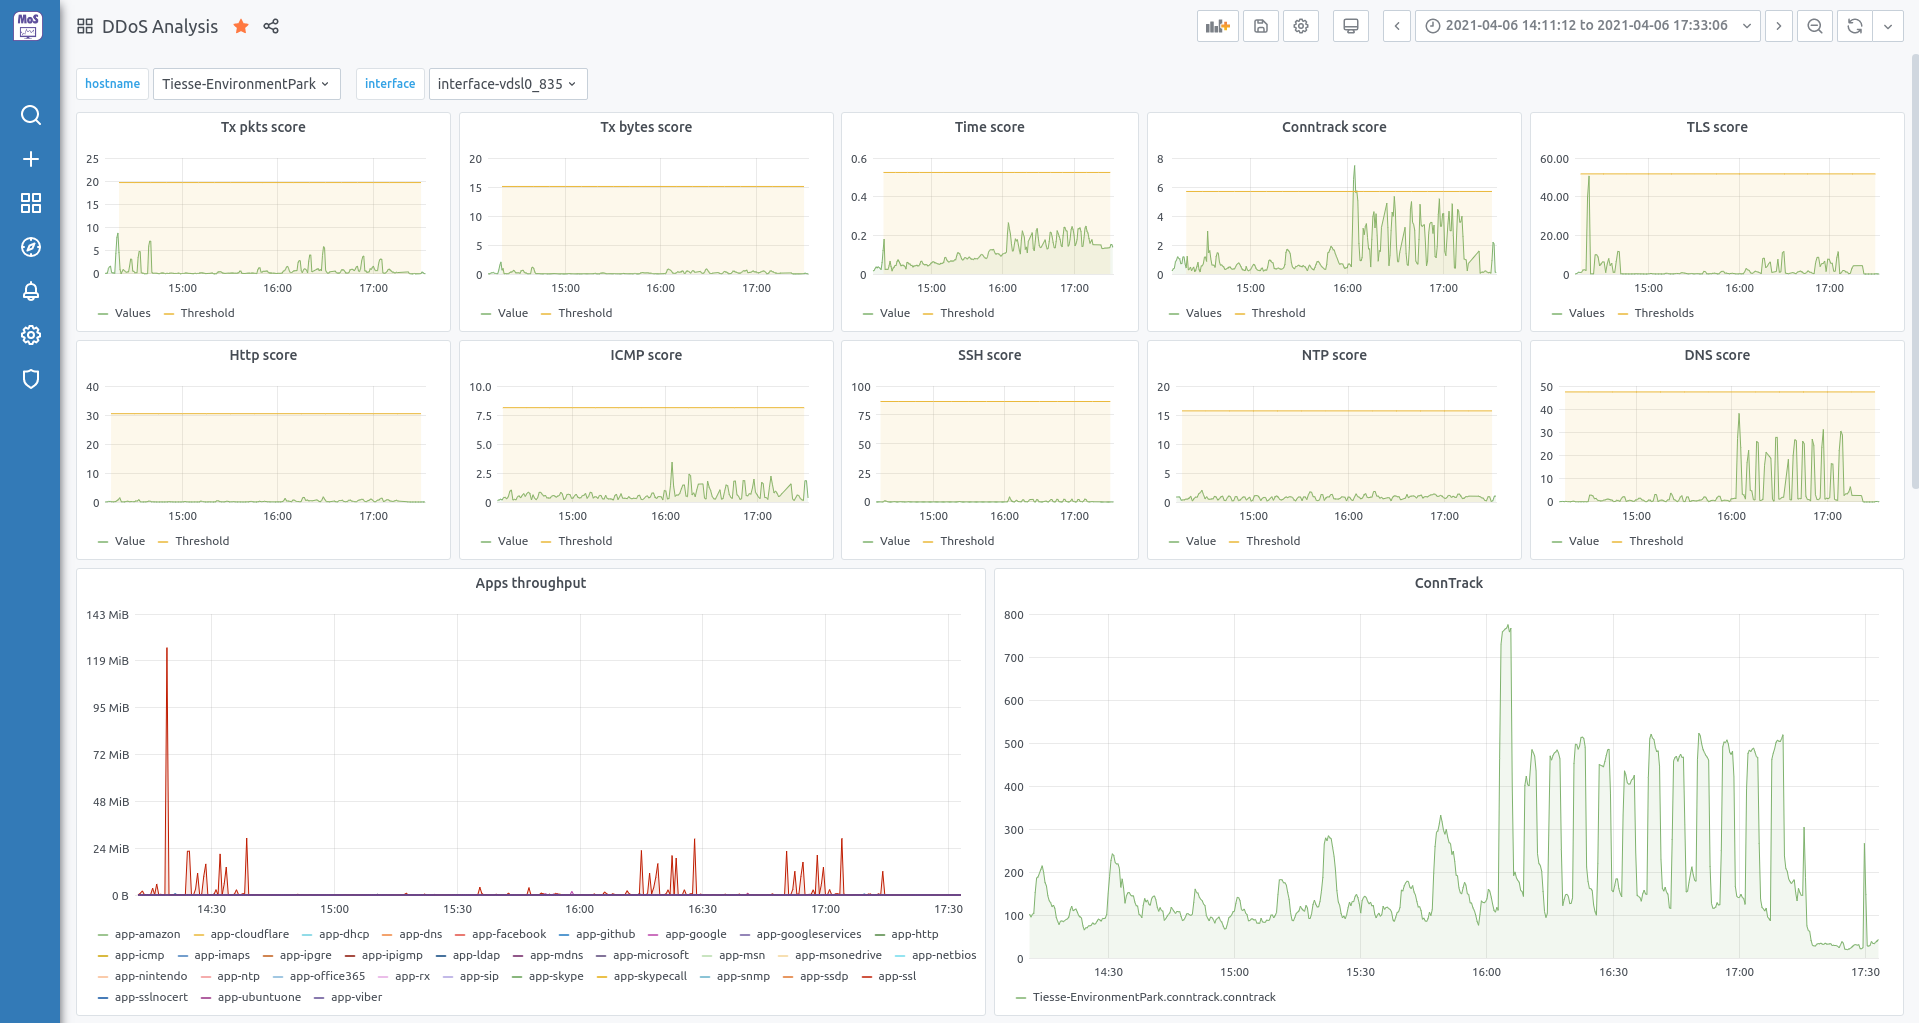
\includegraphics[width=\hsize]{images/my_work/grafana_dashboard.png}
    \caption{La mia dashboard su Grafana}
    \centering
\end{figure}

\paragraph{Grafana} è un software open source che permette la visualizzazione e la generazione delle metriche tramite una web application. Permette di creare dashboard dinamiche interrogando le api di graphite-web. Nel mio caso ho organizzato una dashboard in modo da visualizzare sia i dati provenienti dai router da analizzate, sia gli anomaly score calcolati dal software di anomaly-detection ~\ref{fig:graphana}.


%todo: come vengono mandati i dati di ndpi?
Riassumendo i dati provenienti dai plugin di collect, dal mio plugin e da NDPI vengono collezionati da collectd e inviati tramite il plugin write\_graphite al backend go-carbon, che si occupa di ricevere i dati e salvarli sul file system. Per la visualizzazione dei dati viene usato grafana, che permette di visualizzare i dati richiedendo i dati alle carbonapi e contemporaneamente il mio tool di anomaly detection richiede i dati per analizzarli, ogni volta che ottiene dei risultati li manda a go-carbon per salvarli nel database ~\ref{fig:mos}.
% todo: approfondire MOS
% todo: fare immagine con la gestione dei dati


\section{Selezione features}

La scelta delle feature da utilizzare dipende da quale obiettivo su vuole ottenere, il mio obiettivo primario in questa tesi è di rilevare gli attacchi DDoS in uscita verso la sede centrale, quindi basandomi sugli attacchi più famosi e frequenti ho delineato una lista di parametri da osservare. Questi parametri sono:
% todo: capire le unità di misura i dati sono ogni secondo o ogni 10
\begin{itemize}
    \item \emph{bytes trasmessi al secondo}:questa metrica è utile, abbinata ad altre, per la rilevazione di attacchi che mirano alla saturazione della banda.
    \item \emph{pacchetti trasmessi al secondo}: questa metrica ha uno scopo simile alla precedente oppure aiuta ad avere informazioni sugli attacchi di tipo flooding.
    \item \emph{numero di connessioni aperte}: il numero di connessioni aperte è un indicatore importante per identificare tutti gli attacchi che mirano a saturare le connessioni di un server. %todo: questa ha molti usi
    \item \emph{numero di pacchetti con flag syn}: questa metrica è molto utile per la rilevazione di syn flood o port scanning.
    \item \emph{tls throughput}: tutto il traffico inviato su un canale sicuro tls non può essere analizzato più nello specifico, quindi viene raggruppato in questa categoria.
    \item \emph{dns throughput}: conoscere il traffico relativo al traffico dns può essere utile come indice di un attacco contro il server DNS aziendale oppure di un attacco di DNS amplification.
    \item \emph{ssh throughput}: potrebbe segnalare anomalie sull'utilizzo improprio di macchine nella sede centrale tramite delle connessioni ssh.
    %todo: da rivedere come funzionano gli icmp durante un syn flood
    \item \emph{icmp throughput}: è un indicatore di attacchi, per esempio durante un syn flood usando ip spoofing, con ip della sottorete dell'attaccante, al ritorno dei syn ack si vede un aumento degli icmp che indicano che l'host non è esistente o che la porta destinazione a cui è destinato il pacchetto è chiusa. Inoltre gli icmp possono anche essere usati direttamente per degli attacchi.
    \item \emph{ora del giorno}: l'ora del giorno viene aggiunta per caratterizzare al meglio il traffico lungo la giornata.
    %todo: aggiungere http e ntp
\end{itemize}

Tutte le feature vengono poi \underline{derivate su un tempo di 10/30s, per avere dei "rate"} confrontabili tra lavoro.

La scelta della features è nata da un compromesso tra i dati necessari per rilevare al meglio le anomalie, la riduzione dei dati da salvare sul server e di conseguenza l'uso di banda usata per il trasferimento. Inoltre un problema che ho dovuto tenere in considerazione è l'utilizzo di un \underline{acceleratore hardware} nei router Tiesse, il quale permette un incremento della velocità di routing, ma non permette di analizzare nel kernel i pacchetti.
 %todo: approfondire meglio come funziona il fast path
 
\section{Il mio tool}

Cosa fa?
Perchè l'ho fatto?

Per rilevare le anomalie, una volta decise le features da analizzare, ho dovuto decidere quale sistema dei precedentemente elencati adottare. La scelta è ricaduta sull'utilizzo di una rete neurale di autoencoder, la quale permette di allenare facilmente il modello in modo semi-supervisionato, grazie all'utilizzo della sola classe normale di traffico.

\subsection{Struttura}

Posso parlare di come è strutturato il programma, che librerie ho usato 
Il programma è scritto in Python 3, con l'utilizzo di TensorFlow e Keras librerie per il ``machine learning'', effettua le richieste http tramite la libreria requests e gestisce i dati grazie a NumPy e Pandas: librerie per il calcolo matriciale e la gestione di tabelle e serie.
Il tutto per assicurare una maggiore portabilità, ed assicurare la possibilità di effettuare il deploy su qualsiasi macchina, viene eseguito all'interno di un container Docker, la cui immagine viene creata e avviata tramite ``docker-compose''.


I dati all'interno del repository sono organizzati nel seguente modo:

\dirtree{%
.1 /.
.2 data\DTcomment{Cartella dove verrà salvato il modello e le immagini generate}.
.2 src\DTcomment{Cartella con i sorgenti del programma}.
.3 requirements.txt\DTcomment{Librerie di python necessarie}.
.3 utility.py \DTcomment{File in cui sono presenti le funzioni comuni}.
.3 update\_db.py \DTcomment{Funzioni per caricare i risultati su graphite}.
.3 evaluate.py \DTcomment{File con le funzioni per valutare se sono presenti anomalie}.
.3 train.py \DTcomment{File con funzioni per eseguire l'allenamento della rete}.
.3 model.py \DTcomment{File con funzioni per generare il modello}.
.3 test.py \DTcomment{Script che esegue la creazione di un modello, il train e la successiva valutazione di anomalie, basandosi su un file di impostazioni}.
.3 main.py \DTcomment{Script che esegue la creazione e il train del modello se non presente e a intervalli regolari verifica le anomalie}.
.2 test\_configs.
.3 test\_docs\_v3.json\DTcomment{Un esempio di file di configurazione usato per effettuare i test della validità del modello}.
.2 Dockerfile.
.2 docker-compose.yml.
.2 README.md.
}
\subsection{Keras e TensorFlow}

\paragraph{Tensorflow 2} è una libreria open-source sviluppata da Google per il machine learning che fornisce moduli ottimizzati per la realizzazione di algoritmi di machine learning e la loro esecuzione in maniera efficiente su CPU, GPU e TPU. Inoltre permette di scalare agevolmente su un'architettura con molti device.
% \cite{keras_about}

\paragraph{Keras} è un insieme di API ad alto livello di TensorFlow 2 che forniscono astrazioni essenziali per incentrarsi sulla facilità d'uso, la modularità e l'estendibilità per la risoluzioni di problemi relativi al machine learning, con una particolare concentrazione sui moderni problemi di deep learning.


\subsection{Elaborazione dei dati in input}
Come ricevo i dati dal server? Come li elaboro? Che api uso?
Genero tante piccole sequenze di 8 elementi (spiegare il motivo della scelta della sequence length => trade-off tra tempo di rilevamento dell'anomalia e mitigazione dei picchi e dei falsi positivi) e perchè lo faccio, come normalizzo i dati e perchè. Come fornisco i dati in input alla rete.

Le metriche relative alle applicazioni vengono aggiornate ogni 30 secondi, a differenza dei 10 secondi con cui aggiorno i dati collezionati da collectd, per questo motivo ogni volta che devo richiedere dei dati al server devo effettuare due richieste, tramite la libreria requests, alle carbonapi.

% (Viene usato http con basic auth, questo mi provoca un colpo al cuore lato sicurezza, ma lo posso giustificare dicendo che è un ambiente di test, in produzione come minimo verrà usato https.)

Un esempio di dati che mi restituisce la prima richiesta è (qui per ridurre la quantità di dati ipotizzo che la richiesta sia di 20 secondi):
\begin{lstlisting}[language=json]
[
    {
        "target": "Tiesse-EnvironmentPark.conntrack.conntrack",
        "datapoints": [
            [
                135,
                1619681610
            ],
            [
                134,
                1619681620
            ]
        ],
        "tags": {
            "name": "Tiesse-EnvironmentPark.conntrack.conntrack"
        }
    },
    {
        "target": "Tiesse-EnvironmentPark.interface-vdsl0_835.if_packets.tx",
        "datapoints": [
            [
                21.199091,
                1619681610
            ],
            [
                26.401902,
                1619681620
            ]
        ],
        "tags": {
            "name": "Tiesse-EnvironmentPark.interface-vdsl0_835.if_packets.tx"
        }
    },
    {
        "target": "Tiesse-EnvironmentPark.interface-vdsl0_835.if_octets.tx",
        "datapoints": [
            [
                4202.222148,
                1619681610
            ],
            [
                5862.413248,
                1619681620
            ]
        ],
        "tags": {
            "name": "Tiesse-EnvironmentPark.interface-vdsl0_835.if_octets.tx"
        }
    }
]
\end{lstlisting}

Per elaborare i dati ricevuti devo avere una tabella con il corretto formato, vedi l'esempio di tabella \ref{table:tabella_dati_1}, per questo motivo elaboro i dati del json ricevuto precedentemente, sostituendo per prima cosa il timestamp, trasformandolo da un unix timestamp ad uno che indica i secondi passati dalla mezzanotte e successivamente aggiungo tutti gli elementi ad un json con il corretto formato, come mostrato nell'estratto di codice \ref{code:get_data}.

% todo: e i syn?
\begin{table}[]

\begin{tabular}{||c c c c c||} 
\hline
index & timestamp  & .conntrack.conntrack & ..if\_packets.tx & ..if\_octets.tx \\ [0.5ex] 
\hline\hline
1 & 45810 & 71.0 & 7.500424 & 2416.445886 \\ 
\hline
2 & 45820 & 74.0 & 4.89923 & 51069.831629415 \\
\hline
3 & 45830 & 72.0 & 5.000281 & 1224.055123 \\
\hline
\end{tabular}
\caption{Tabella di esempio dei dati ricevuti relativi alle features di collect.}
\label{table:tabella_dati_1}
\end{table}
% \begin{lstlisting}[language=csv]
% ,timestamp,.conntrack.conntrack,..if_packets.tx,..if_octets.tx
% 0,45810,181.0,38.902328,6055.20679
% 1,45810,181.0,38.902328,6055.20679
% \end{lstlisting}

% todo: come metto le lettere accentate?
\begin{lstlisting}[language=Python, label={code:get_data}, caption={Funzione usata per scaricare i dati dal server}]
def get_data(s_time, e_time, hostname: str, interface: str,
    username: str = None, password: str = None):

    r = requests.get(
    f"http://{host}:{port}/api/datasources/proxy/4/render?"
    f"target={'&target='.join(target_list(hostname,interface))}"
    f"&from={s_time}&until={e_time}&format=json",
    auth=HTTPBasicAuth(username, password)
    )

    # se il valore ritornato non e' un'eccezione,
    # che verra' gestita a livelli superiori
    print(r.status_code, '-', r.url)
    if r.status_code != 200:
    raise Exception('Get features data error')


    # converto la risposta in un json 
    # e poi in un dizionario con chiave il target
    # e come valore i datapoints
    json_resp = r.json()

    # todo: probabilmente ci sono modi piu' efficienti
    data = data_to_dict(json_resp)
    data_list = list()
    for i in range(len(json_resp[0]['datapoints'])):
        line: dict = dict()
        timestamp =
        datetime.fromtimestamp(json_resp[0]['datapoints'][i][1])
        # trasformo il tempo in secondi dalla mezzanotte
        line['timestamp'] = timestamp.hour * 3600 \
                            + timestamp.minute * 60 \
                            + timestamp.second
        tl = target_list(hostname, interface)
        for e in tl:
            line[e] = data[e][i][0]
        data_list.append(line)

    # creo la matrice con pandas ed elimino le righe con valori
    # mancanti in rari casi le carbon api mi restituiscono dei
    # valori nulli, per questo motivo cancello le righe in cui
    # c'e' almeno un valore nullo
    matrix = pd.DataFrame(data_list).dropna()

    # successivamente richiedo anche i dati delle app, e quando
    # li ricevo, dopo averli manipolati, li unisco tutti
    # in un'unica tabella
    app_data_matrix =
    get_app_data(s_time, e_time, hostname, username, password)

    matrix = pd.merge(app_data_matrix, matrix)

    # questa funzione mi permette di ritornare l'elenco 
    # delle feature attualmente utilizzate, senza impostare
    # host e interfaccia da utilizzare
    matrix.columns = total_target_list('', '')
    return matrix

\end{lstlisting}

Una volta ricevuti i dati e organizzati nel formato corretto, effettuo una nuova richiesta alle carbon api, per ricevere i dati relativi alle applicazioni, il procedimento è simile a quello precedentemente descritto, l'unica differenza è che estendo i dati, mostrando lo stesso dato più volte, in modo da avere lo stesso numero di elementi ottenuti precedentemente.

\begin{lstlisting}[language=Python]
for element in app_list:
    # se l'app non esiste nella risposta metto uno 0
    line[element] =
     data[element][i][0] if element in data else 0.0
# estendo i dati, replicando lo stesso dato ogni 10s per un totale di 30s
for j in range(3):
    line['timestamp'] += 10
    data_list.append(line.copy())
\end{lstlisting}

\paragraph{La standardizzazione dei dati} è la fase subito successiva, 
% differenziare i casi tra l'evaluate e il train
Durante il train calcolo la media e la deviazione standard sui dati per ogn, successivamente standardizzo e salvo la media e deviazione standard di ogni feature su un file.
Durante la fase di evaluate per standardizzare i dati uso i dati salvati precedentemente sul file e standardizzo i dati.
% Un problema della standardizzazione dei dati è la gestione dei picchi le reti neurali lavorano meglio con dati piccoli, quindi i picchi potrebbero essere un problema, si può pensare un modo diverso per standardizzare i dati

\paragraph{Scelta della lunghezza delle sequenze dei dati.} Utilizzando i dati standardizzati genero ``N-K'' sequenze di lunghezza ``K'' elementi, dove ``N'' è il numero di elementi ricevuti precedentemente. Queste sequenze mi servono per uniformare i dati di allenamento e valutazione usando una lunghezza fissa per la sequenza di dati da dare in input alla rete neurale.
La scelta della lunghezza della sequenza è molto importante, perchè da essa dipende la capacità di rilevamento delle anomalie: più il valore sarà grande e più sarà preciso il riconoscimento delle anomalie e meno il programma sarà soggetto a falsi positivi, ma al tempo stesso renderà di difficile identificazione i picchi anomali e il tempo necessario per rilevare un'anomalia sarà maggiore.
%todo: aggiungo il codice per creare le sequenze?
%todo: qua spiego cosa ho scelto allegando delle immagini
Abbiamo scelto una lunghezza della sequenza di otto elementi
%https://keras.io/examples/timeseries/timeseries_anomaly_detection/

\subsection{Modello della rete}

Spiego come ho usato Keras per generarlo.
Spiego come sono arrivato a scegliere il modello e comparo i risultati tra 2/3 modelli totalmente diversi come numero di nodi, sarebbe interessante provare a mettere anche un modello con retroazione visto che stiamo usando sequenze temporali.

Il modello di una rete neurale serve a descrivere le interconnessioni, le diverse tipologie e la composizione dei livelli di una rete neurale, è un oggetto della libreria Keras, che può essere facilmente creato grazie alla funzione ``tf.keras.Model()''.
Nel nostro caso ogni livello prevedeva un solo livello in ingresso e uno in uscita, per questo motivo abbiamo usato il ``sequential model'' di Keras.
La nostra rete è composta da un semplice autoencoder a cinque livelli: uno di input e uno di output con dimensioni (lunghezza\_sequenza, numero\_features) e livelli con prima una riduzione e poi un incremento dei nodi, come nei classici autoencoders.
Avendo in ingresso dei dati con più dimensioni ho dovuto linearizzare i dati in ingresso (flatten) e ricostruire il vettore multidimensionale in uscita (reshape), nei nodi intermedi invece ho usato progressivamente un layer con 25 nodi, uno spazio latente con 8 e un livello successivo di nuovo con 25 nodi. La scelta delle dimensioni dei livelli centrali è stata presa analizzando più configurazioni e considerando che usando una lunghezza della sequenza di otto elementi, con dieci features significa avere 80 nodi in input e output, di conseguenza i nodi nei livelli centrali devono essere meno.
Per creare la rete sono stati usati ``Dense layers'', in cui cui i nodi di due livelli sono interamente connessi tra loro e sono state usate come funzioni di attivazioni ``relu'' (Equazione \ref{eq:relu}) per i nodi intermedi e ``linear'', una funzione lineare, per i nodi dell'ultimo livello, questo permette di rappresentare anche i numeri negativi.
%https://keras.io/api/models/model/

\begin{equation} \label{eq:relu}
    f(x) = x^+ = max(0, x)
\end{equation}

Il modello viene infine compilato e salvato su file, in modo da potere essere usato successivamente.

\begin{lstlisting}[language=Python, label={code:get_data}, caption={Funzione usata per generale il modello della rete neurale}]
    sequential_model = keras.Sequential(
        [
            layers.Flatten(input_shape=shape),
            layers.Dense(25, activation='relu'),
            layers.Dropout(rate=0.2),
            layers.Dense(8, activation='relu'),
            layers.Dropout(rate=0.2),
            layers.Dense(25, activation='relu'),
            layers.Dropout(rate=0.2),
            layers.Dense(shape[1]*shape[0], activation='linear'),
            layers.Reshape((shape[0], shape[1]))

        ]
    )
\end{lstlisting}

\subsection{Train}
Il train deve essere effettuato su degli intervalli di tempo in cui non si sono verificate anomalie, per questo motivo viene fatta l'assunzione che tutto il traffico generato non presenti anomalie a meno di piccoli intervalli in cui è stato volutamente generato traffico malevolo per scopo di test. Volendo se l'amministratore di sistema notasse altri periodi di traffico anomalo potrà escluderli dai dati di allenamento.
Inoltre per avere un maggiore numero di dati, e velocizzare l'apprendimento dell'allenamento della rete, è possibile utilizzare i dati provenienti da più router delle sedi periferiche, se ipotizziamo che il traffico generato sia simile tra loro.
Dalla selezione degli intervalli di tempo su cui si vuole effettuare il train per semplicità in questa prima versione di algoritmo vengono esclusi i weekend: giorni della settimana in cui, nel nostro caso, il traffico è molto diverso dagli altri, volendo risolvere il problema si potrebbe usare una seconda rete da usare solo nei giorni festivi o %todo: proporre altre soluzioni per i weekend
Nella fase di train per prima cosa verrà effettuato la raccolta e la trasformazione dei dati dal server, come spiegato precedentemente e avere caricato da file il modello generato.
Successivamente prima di effettuare il train vero e proprio, grazie alla funzione ``train\_test\_split'' della libreria sklearn i dati vengono divisi in due insiemi, quello di train e quello di test, con il 15\% dei dati usati per il test e il restante per il train.
L'allenamento viene effettuato usando il metodo ``fit'' della classe model e usando in input sia per le x, che per le y, l'insieme di train appena generato e l'insieme di test per validare il modello. Inoltre è abilitato l'EarlyStopping, in cui se per più di cinque iterazioni non si hanno miglioramenti, viene stoppato il processo di allenamento, questo serve per ridurre i tempi di train e ridurre la possibilità di overfitting.
%todo: da valutare possibilità di overfitting.

Come spiegato precedentemente, l'utilizzo degli autoencoders permette di ottenere degli ``anomaly score'' per ogni sequenza di dati, quindi terminata la fase di allenamento della rete devo decidere sopra quale valore devo considerare i dati anomali.
Le soglie sopra i quali considero i dati anomali vengono prese dal massimi valore degli anomaly score per ogni feature: avendo ipotizzato che tutti i dati forniti per il train non siano anomali, devo assicurarmi che effettuando la valutazione delle anomalie su quei dati nulla risulti anomalo.
% todo: potrei anche aumentare le soglie di un certo valore per essere meno soggetto a falsi positivi
Per calcolare l'anomaly score calcolo il valore medio dei valori assoluti delle differenze tra il valore originale e quello ricostruita.
\begin{equation}
    % \caption{Formula per il calcolo dell'anomaly score}
    anomaly\_score = \frac{\sum_{elementi\_sequenza}\lvert valore\_originale - valore\_ricostruito \rvert}{lunghezza\_sequenza}
\end{equation}
Le soglie calcolate vengono salvate su un file, da potere usare successivamente per la valutazione delle anomalie.

Quando eseguire il train?
% todo: per quanto tempo faccio il train? 

%todo: Immagini di confronto dei valori ricostruiti e originali con anomalie e non


% Come effettuo il train?
% Quali dati uso?
% Cosa escludo? 
% Per quanto tempo?
% e se il traffico varia nel tempo?
% Vantaggi e svantaggi del train fatto in questo modo
% Overfitting? 

% Assumo che gli intervalli di traffico utilizzati per il train non includa anomalie, que
% Utilizzo il traffico di più uffici per velocizzare l'apprendimento se hanno caratteristiche simili

% Scartati i weekend perchè i dati sono molto diversi rispetto al resto della settimana e la rete non tiene in considerazione il giorno della settimana.

\subsection{Evaluate}
% Come effettuo la valutazione? Su quali sequenze?
Allenato il modello a ricostruire l'input e calcolate sopra le quali considerare gli anomaly score anomali è possibile verificare se il traffico generato in un intervallo di tempo da un determinato router è anomalo.  
Per mettere in atto questa fase, dopo avere trattato i dati in ingresso nello stesso modo dei dati per l'allenamento, leggo dal file generato precedentemente le soglie e verifico se ogni sequenza di k elementi è anomala, calcolando gli anomaly score come effettuato nell'ultima fase del train. Se gli anomaly score superano le soglie si è verificata un'anomalia, a questo punto viene segnalata all'amministratore di rete e viene attivata la fase di mitigazione sul router.
% come viene attivata questa fase? C'è una comunicazione tra server e router?
Questa fase viene ripetuta automaticamente dal software ogni periodo di tempo definito (nell'ordine dei trenta secondi) per i dati di ogni router di cui si vogliono monitorare le anomalie.

\section{Test sulle anomalie}

L'analisi delle anomalie in questa tesi ha l'obiettivo principale di rilevare attacchi DDoS, quindi basandoci sullo studio degli attacchi più popolari abbiamo selezionato un ristretto elenco di attacchi possibili da riprodurre:
%todo: noi l'abbiamo fatto da una sorgente sola, quindi alla fine è un dos, dobbiamo aggregare maggiormente i dati per capire se si tratta di un ddos?
%todo: la feature ssh non sono convinto che sia utile, nel nostro caso è usata talmente poco che temo sia quasi dannosa (viene usata per ricostruire meglio le altre metriches)
\begin{itemize}
    \item SYN flood
    \item ICMP flood
    \item UDP flood
    \item DNS flood
    \item DNS amplification
\end{itemize}

\subsection{Tool utilizzati}

Per effettuare le varie tipologie di attacchi sono stati usati software open-source reperibili sul web e sono stati scritti dei tool per adeguarsi al meglio alle nostre esigente.

\paragraph{hping3} è un tool in grado di generare pacchetti di rete TCP/IP personalizzati. Il nostro utilizzo è stato per generare attacchi di tipo SYN flood, ICMP flood e UDP flood. Il tool, oltre a permettere di generare i pacchetti personalizzati da mandare alla vittima, permette di regolare la portata dell'attacco, tramite le possibilità di sceltà del rate a cui inviare i pacchetti.
% https://linux.die.net/man/8/hping3

Per cosa è stato usato, quali sono i limiti di hping3 e perchè dobbiamo

\paragraph{Il nostro toool}
Parlare come funzionano i tool che ho fatto

\subsection{Risultati}
